\section{Random Forest}
Per l'addestramento è stato utilizzato il package R \texttt{RandomForest}.

\subsection{Holdout}
La stima degli errori di classificazione OOB è del 7,06\%.\\

Le misure di accuracy, precision, recall e F-measure sono le seguenti:
\begin{figure}[H]
	\centering
	\begin{tabular}{lcccc}
		\toprule
		& \textbf{Accuracy} & \textbf{Precision} & \textbf{Recall} & 
		\textbf{F-Measure}  \\
		\midrule
		Training	& 94,41\% & 87,63\% & 38,65\% & 53,64\%    	\\ 
		Validation	& 93,11\% & 70,41\% & 28,33\% & 40,41\%   	\\ 
		\bottomrule
	\end{tabular}
	\captionof{table}{Analisi performance dell'holdout}
	\label{tab:rf_h_performance}
\end{figure}

Di seguito vengono mostrate le curve ROC per il training e il validation set:

\begin{figure}[H]
	\centering
	\begin{subfigure}[t]{1\textwidth}
		\begin{minipage}[t]{0.475\textwidth}
			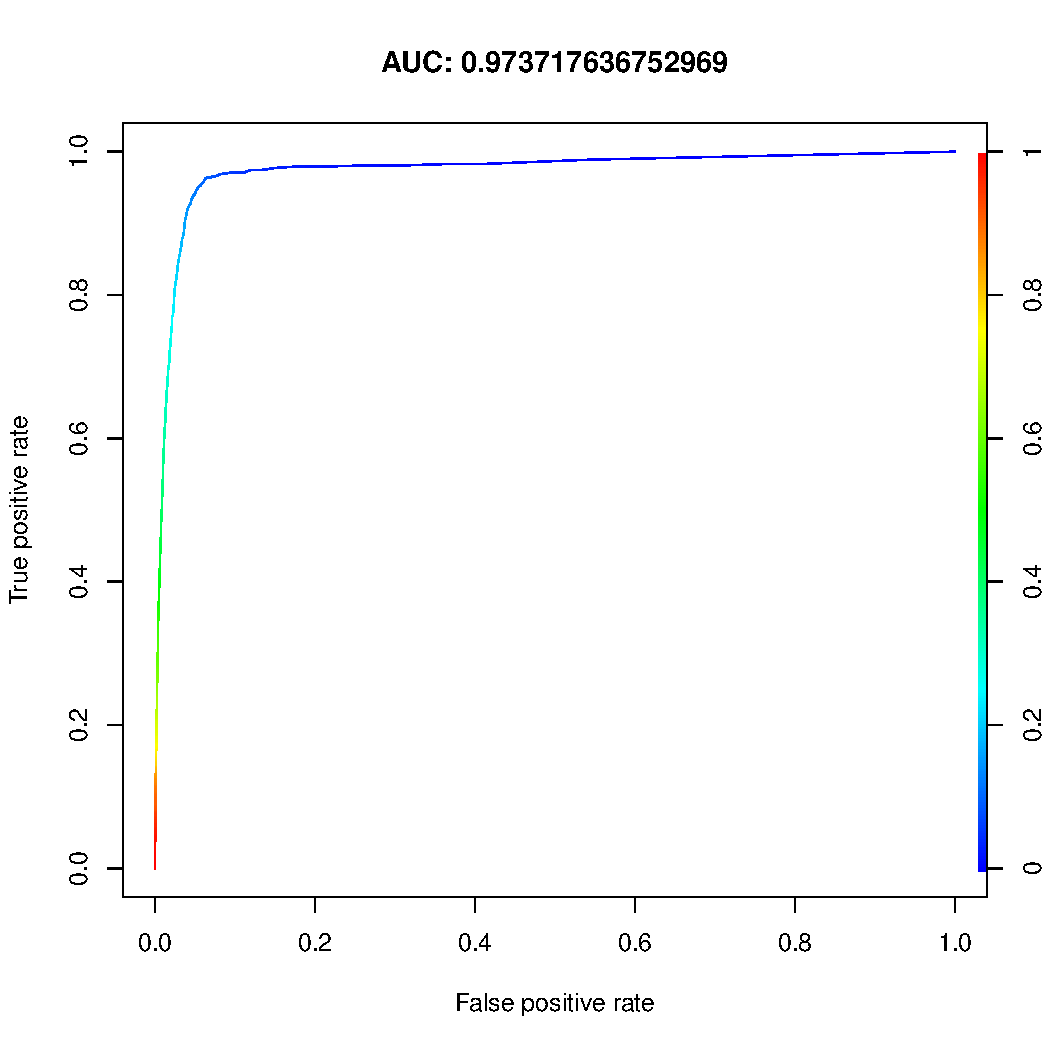
\includegraphics[width=\textwidth]{images/ml/random_forest/HoldoutRF/auc_train}
		\end{minipage}
		\hfill
		\begin{minipage}[t]{0.475\textwidth}
			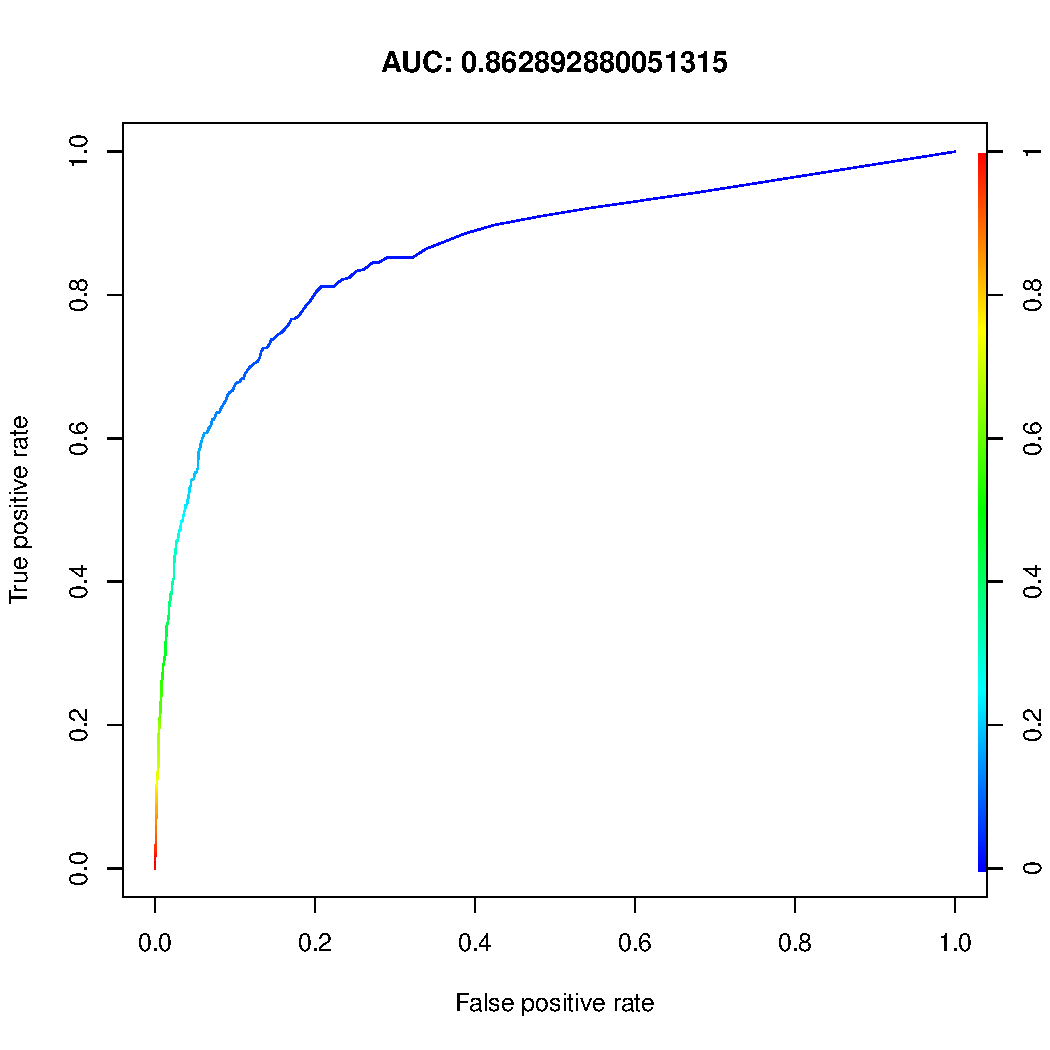
\includegraphics[width=\textwidth]{images/ml/random_forest/HoldoutRF/auc_test}
		\end{minipage}
	\end{subfigure}
	\caption{ROC sul training e validation set}
	\label{fig:rf_h_roc}
\end{figure}


\subsection{10-fold Cross Validation}
La stima degli errori di classificazione OOB è del 7,06\%, ed stata calcolata 
come la media della misura su ogni fold.

Vengono mostrate nella tabella \ref{tab:rf_cv_OOB} la stima degli errori OOB 
per ogni fold.

\begin{figure}[H]
	\centering
	\begin{tabular}{lcccccccccc}
		\toprule
		Fold & \textbf{1} & \textbf{2} & \textbf{3} & \textbf{4} & 
		\textbf{5} & \textbf{6} & \textbf{7} & \textbf{8} & 
		\textbf{9} & \textbf{10} \\
		\midrule
		&7,22\% & 7,32\% & 7,25\% & 7,36\% & 7,01\% & 7,29\% & 6,78\% & 6,84\% 
		& 6,82\% & 6,75\%  	\\ 
		\bottomrule
	\end{tabular}
	\captionof{table}{Stima degli errori di classificazione OOB}
	\label{tab:rf_cv_OOB}
\end{figure}

Per quanto riguarda le misure finali di accuracy, precision, recall e 
f-Measure, come per l'errore di classificazione OOB sono state calcolare come 
la media delle misure su ogni fold. 
Vengono mostrate nella tabella \ref{tab:rf_cv_fold_performance} i dati relativi 
ad ogni fold e in tabella \ref{tab:rf_cv_performance} le misure complessive.

\begin{figure}[H]
	\centering
	\begin{tabular}{llcccc}
		\toprule
		&& \textbf{Accuracy} & \textbf{Precision} & \textbf{Recall} & 
		\textbf{F-Measure}  \\
		\midrule
		\multirow{10}{*}{Training} & Fold1 & 94,23\% & 84,42\% & 40,57\% & 
		54,80\% \\
		& Fold2 & 94,43\%  & 84,30\% & 43,81\% & 57,65\% \\
		& Fold3 & 94,17\%  & 85,68\% & 37,93\% & 52,59\% \\
		& Fold4 & 94,09\%  & 85,98\% & 39,02\% & 53,68\% \\
		& Fold5 & 94,38\%  & 85,22\% & 39,86\% & 54,32\% \\
		& Fold6 & 93,99\%  & 85,52\% & 37,46\% & 52,10\% \\
		& Fold7 & 94,53\%  & 85,00\% & 36,83\% & 51,40\% \\
		& Fold8 & 94,72\%  & 87,09\% & 40,01\% & 54,83\% \\
		& Fold9 & 94,37\%  & 84,93\% & 35,51\% & 50,08\% \\
		& Fold10 & 94,50\% & 86,60\% & 35,77\% & 50,63\%  \\
		\midrule
		\multirow{10}{*}{Validation} & Fold1 & 94,51\% & 78,57\% & 7,43\% & 
		13,58\% \\
		& Fold2 & 94,78\% & 75,00\% & 6,47\% & 11,92\% \\
		& Fold3 & 94,62\% & 92,11\% & 20,71\% & 33,82\% \\
		& Fold4 & 95,68\% & 57,14\% & 10,62\% & 17,91\% \\
		& Fold5 & 92,35\% & 63,64\% & 6,97\% & 12,55\% \\
		& Fold6 & 95,45\% & 76,92\% & 8,13\% & 14,71\% \\
		& Fold7 & 88,85\% & 66,14\% & 25,85\% & 37,17\% \\
		& Fold8 & 90,93\% & 73,55\% & 30,90\% & 43,52\% \\
		& Fold9 & 89,29\% & 58,71\% & 30,33\% & 40,00\% \\
		& Fold10 & 89,76\% & 66,67\% & 36,36\% & 47,06\% \\
		\bottomrule 
	\end{tabular}
	\captionof{table}{Analisi di performance per ogni fold}
	\label{tab:rf_cv_fold_performance}
\end{figure}

\begin{figure}[H]
	\centering
	\begin{tabular}{lcccc}
		\toprule
		& \textbf{Accuracy} & \textbf{Precision} & \textbf{Recall} & 
		\textbf{F-Measure}  \\
		\midrule
		Training	&  94,34\% & 85,47\% & 38,68\%	& 53,21\%  	\\ 
		Validation	&  92,62\% & 70,85\% & 18,38\%	& 27,22\%	\\ 
		\bottomrule
	\end{tabular}
	\captionof{table}{Analisi performance cross validation}
	\label{tab:rf_cv_performance}
\end{figure}

Vengono infine mostrate le curve ROC per ognuno dei fold, sia sul traning che 
sul validation set:

%\begin{figure}[htb]
%	
%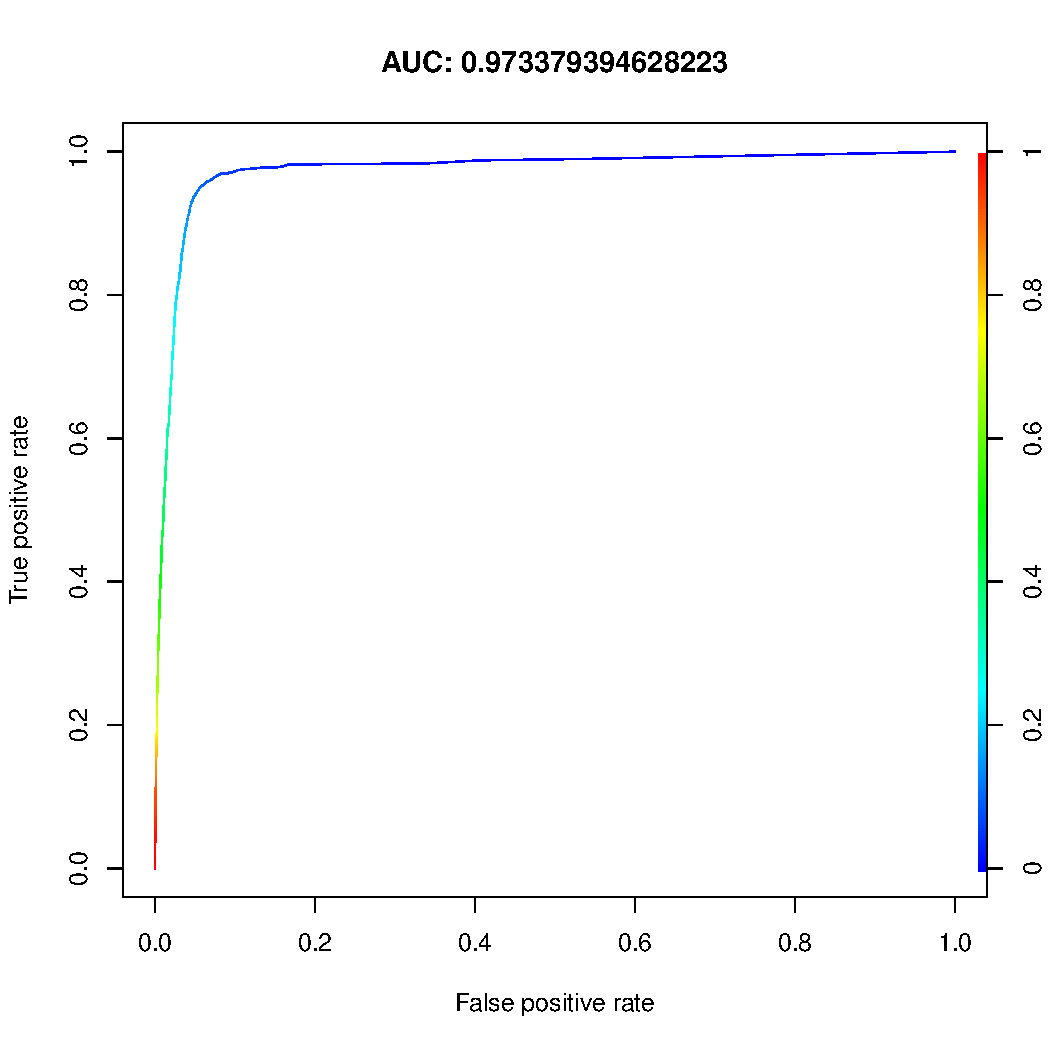
\includegraphics[width=.25\textwidth]{images/ml/random_forest/CrossValidationRF/train/auc_1}
%	
%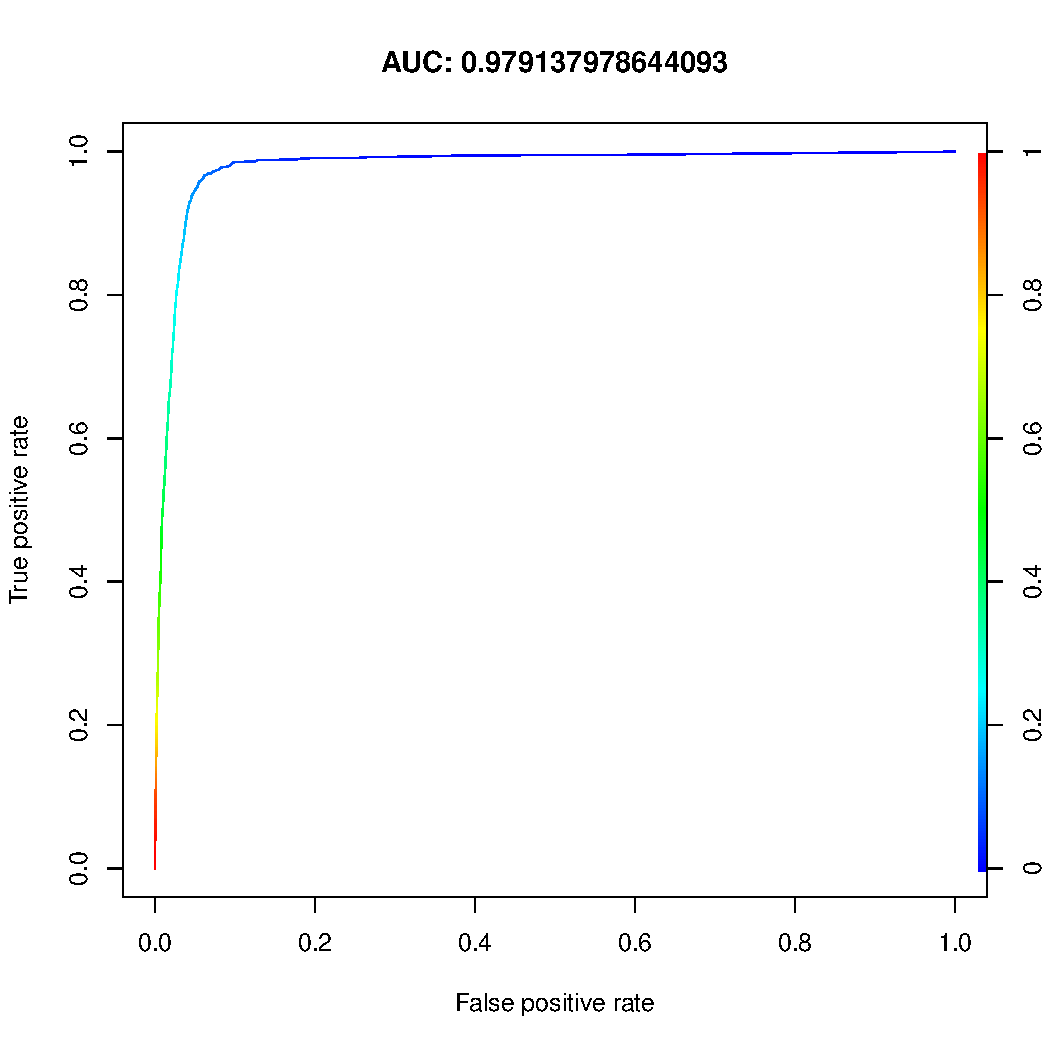
\includegraphics[width=.25\textwidth]{images/ml/random_forest/CrossValidationRF/train/auc_2}
%	
%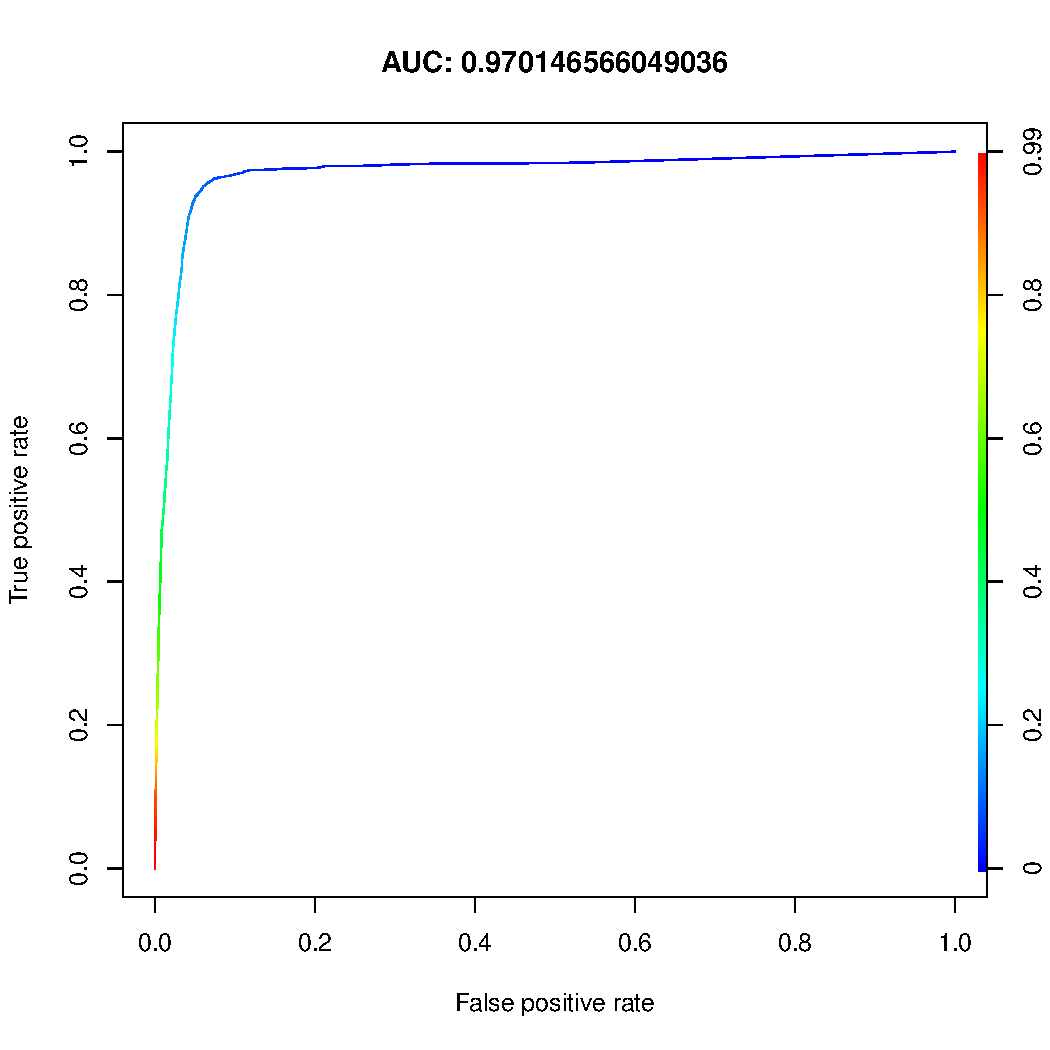
\includegraphics[width=.25\textwidth]{images/ml/random_forest/CrossValidationRF/train/auc_3}
%	
%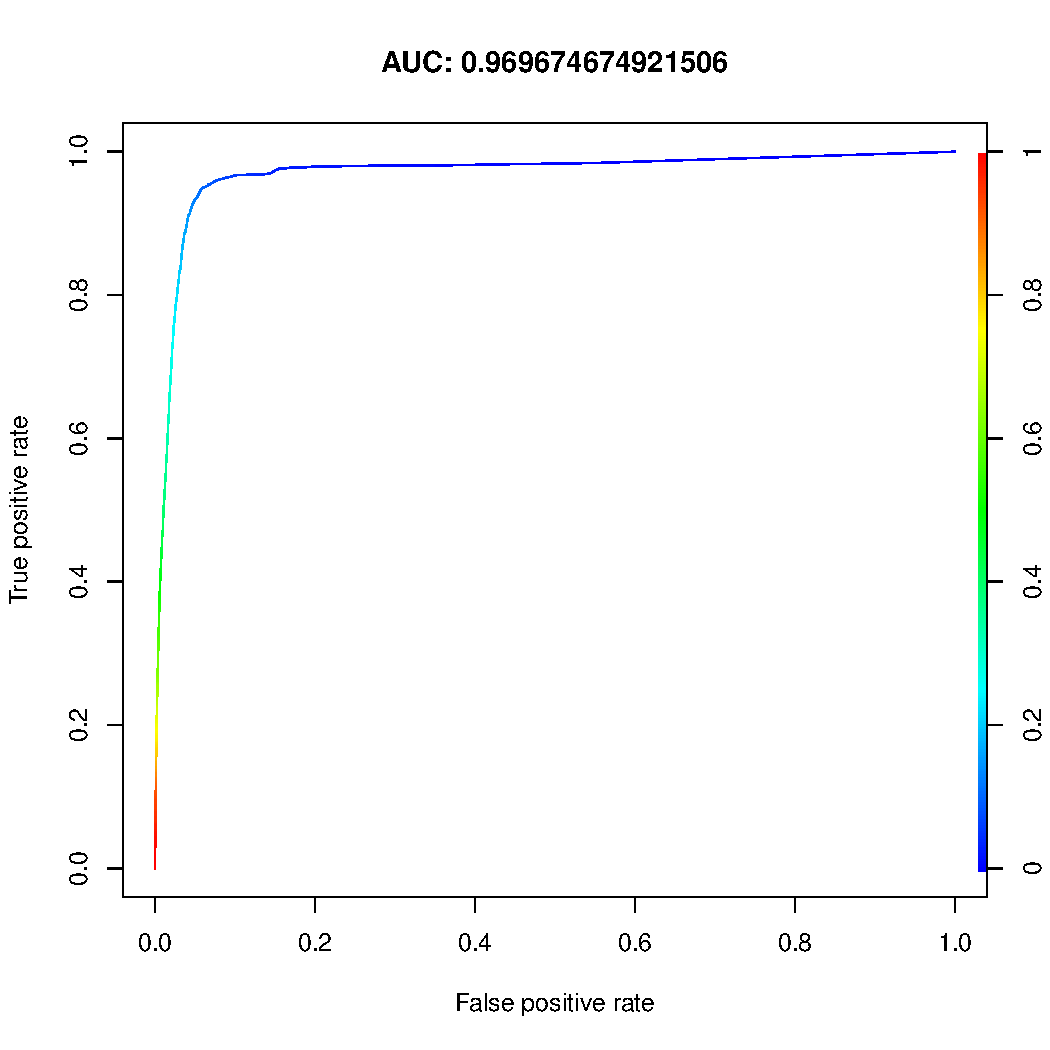
\includegraphics[width=.25\textwidth]{images/ml/random_forest/CrossValidationRF/train/auc_4}
%	
%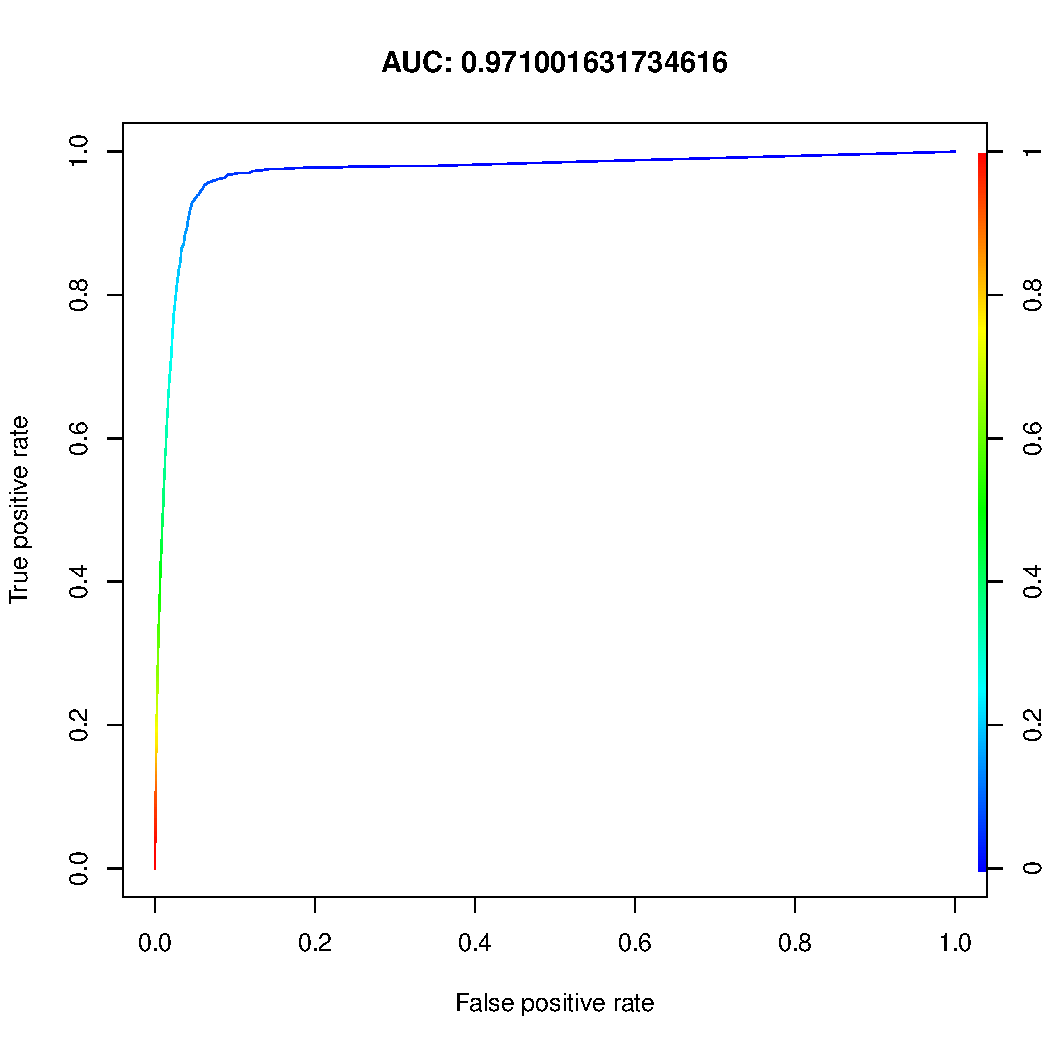
\includegraphics[width=.25\textwidth]{images/ml/random_forest/CrossValidationRF/train/auc_5}
%	
%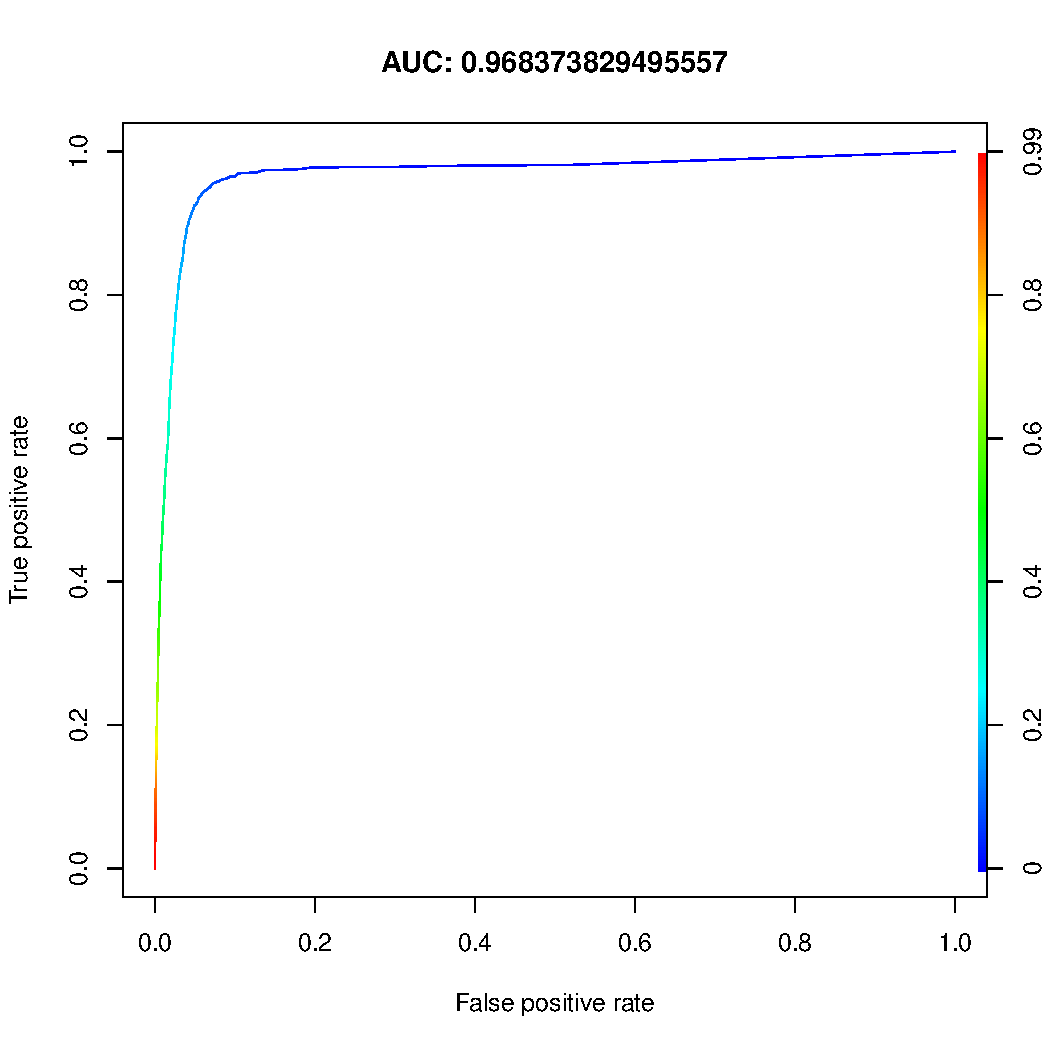
\includegraphics[width=.25\textwidth]{images/ml/random_forest/CrossValidationRF/train/auc_6}
%	
%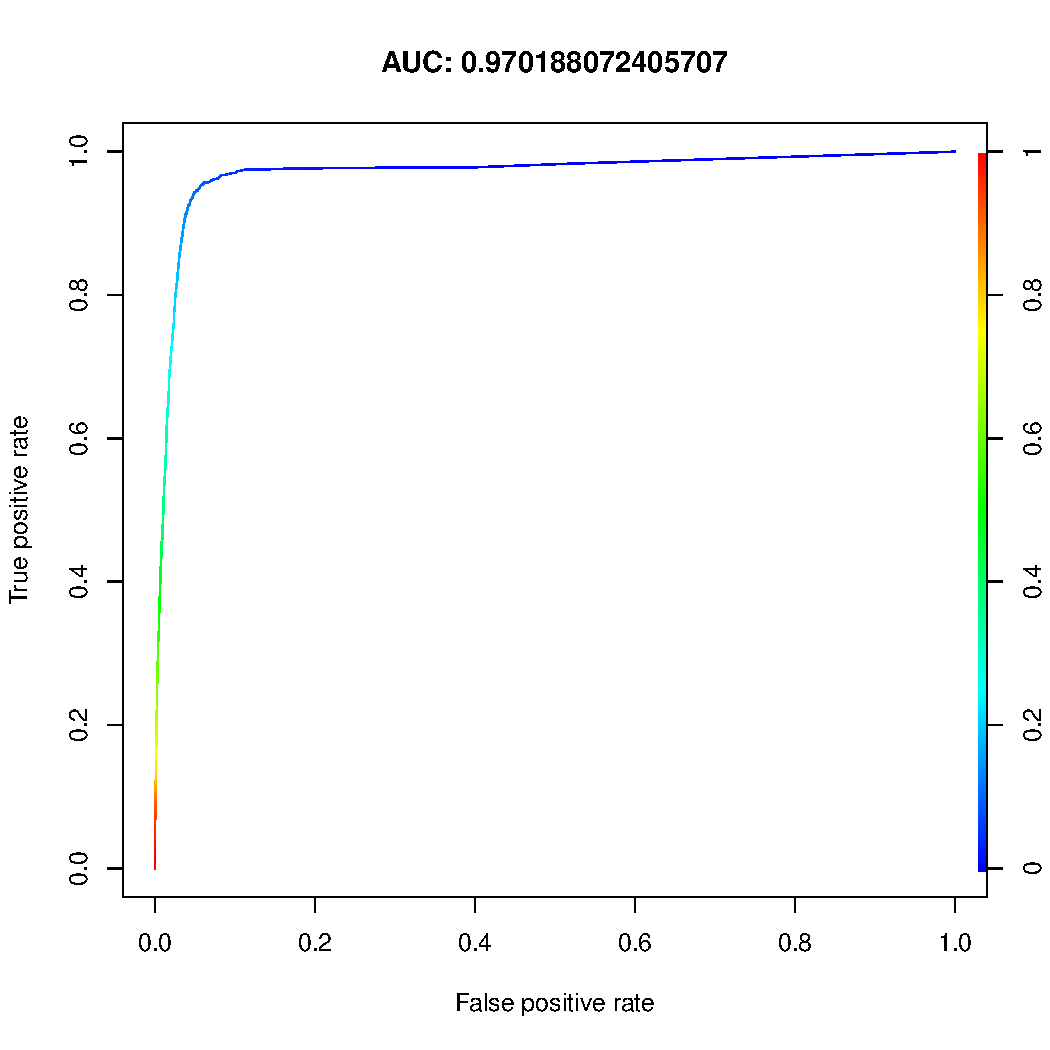
\includegraphics[width=.25\textwidth]{images/ml/random_forest/CrossValidationRF/train/auc_7}
%	
%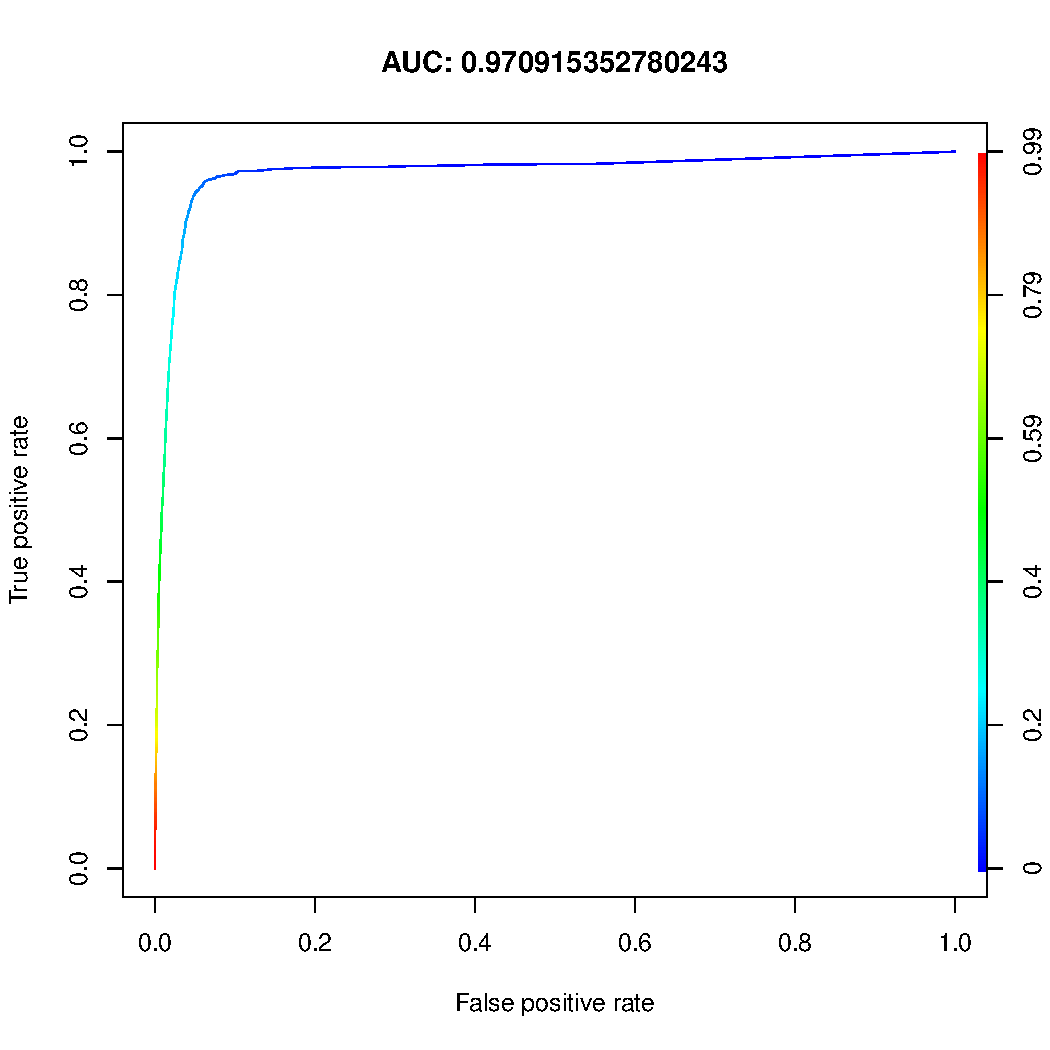
\includegraphics[width=.25\textwidth]{images/ml/random_forest/CrossValidationRF/train/auc_8}
%	
%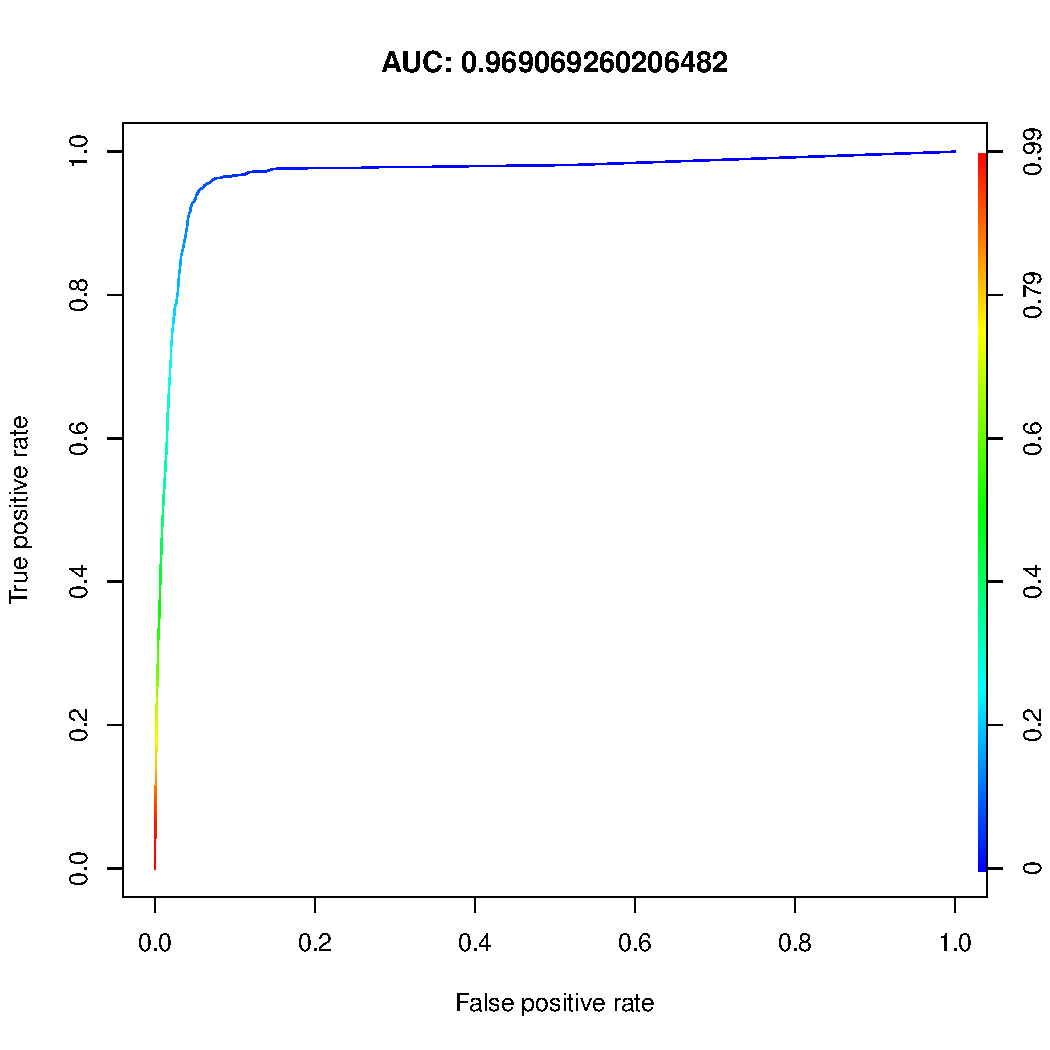
\includegraphics[width=.25\textwidth]{images/ml/random_forest/CrossValidationRF/train/auc_9}
%	
%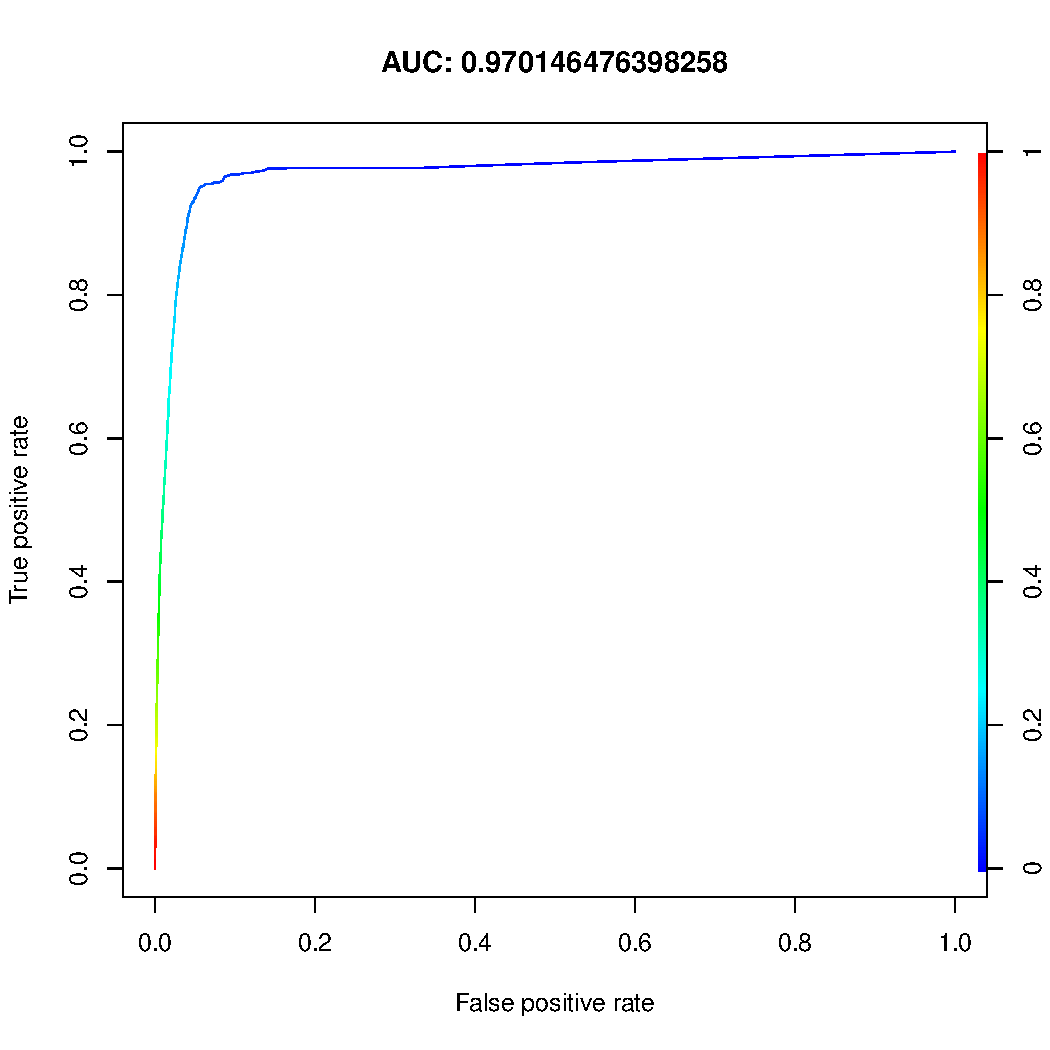
\includegraphics[width=.25\textwidth]{images/ml/random_forest/CrossValidationRF/train/auc_10}
%	\caption{ROC sul training set}
%	\label{fig:rf_cv_roc_train}
%\end{figure}

\begin{figure}[p]
	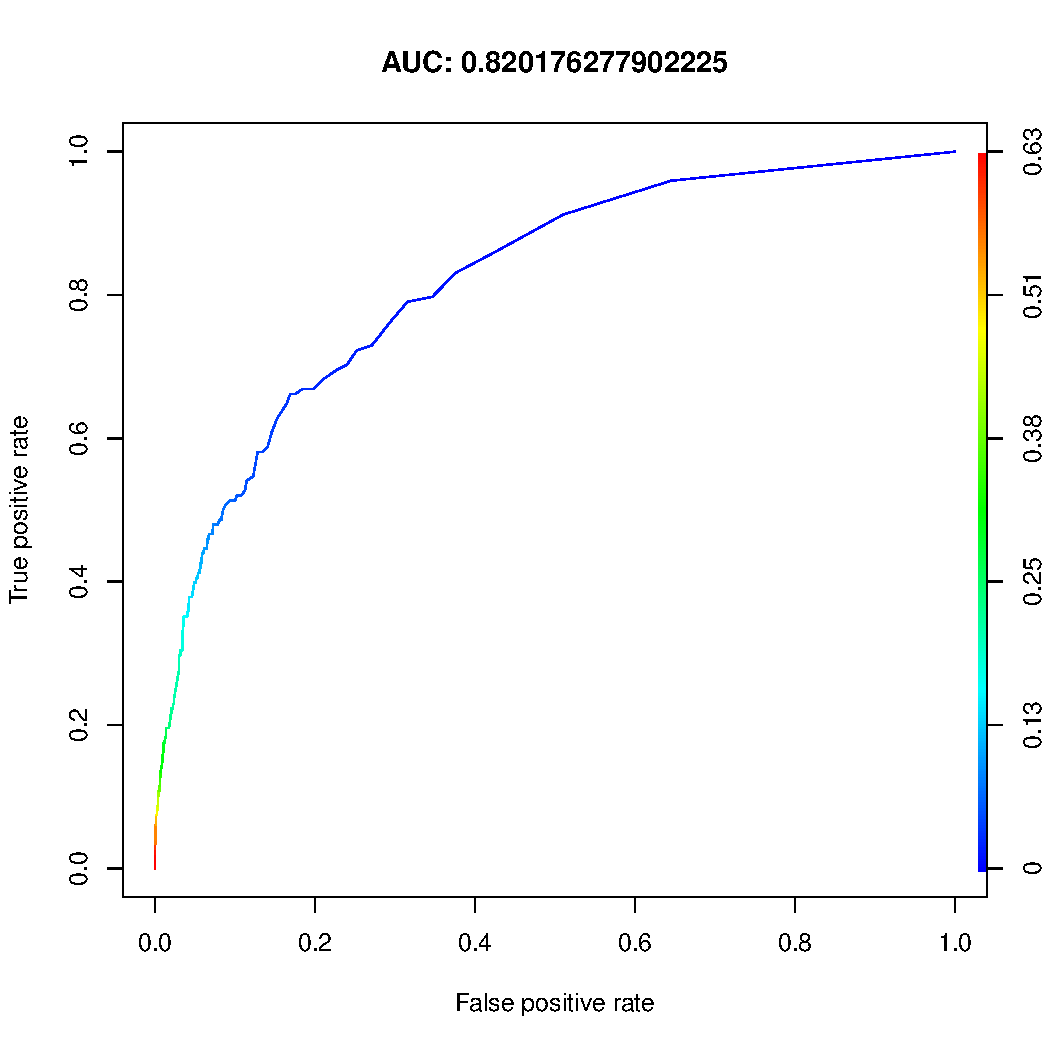
\includegraphics[width=.32\textwidth]{images/ml/random_forest/CrossValidationRF/valid/auc_1}
	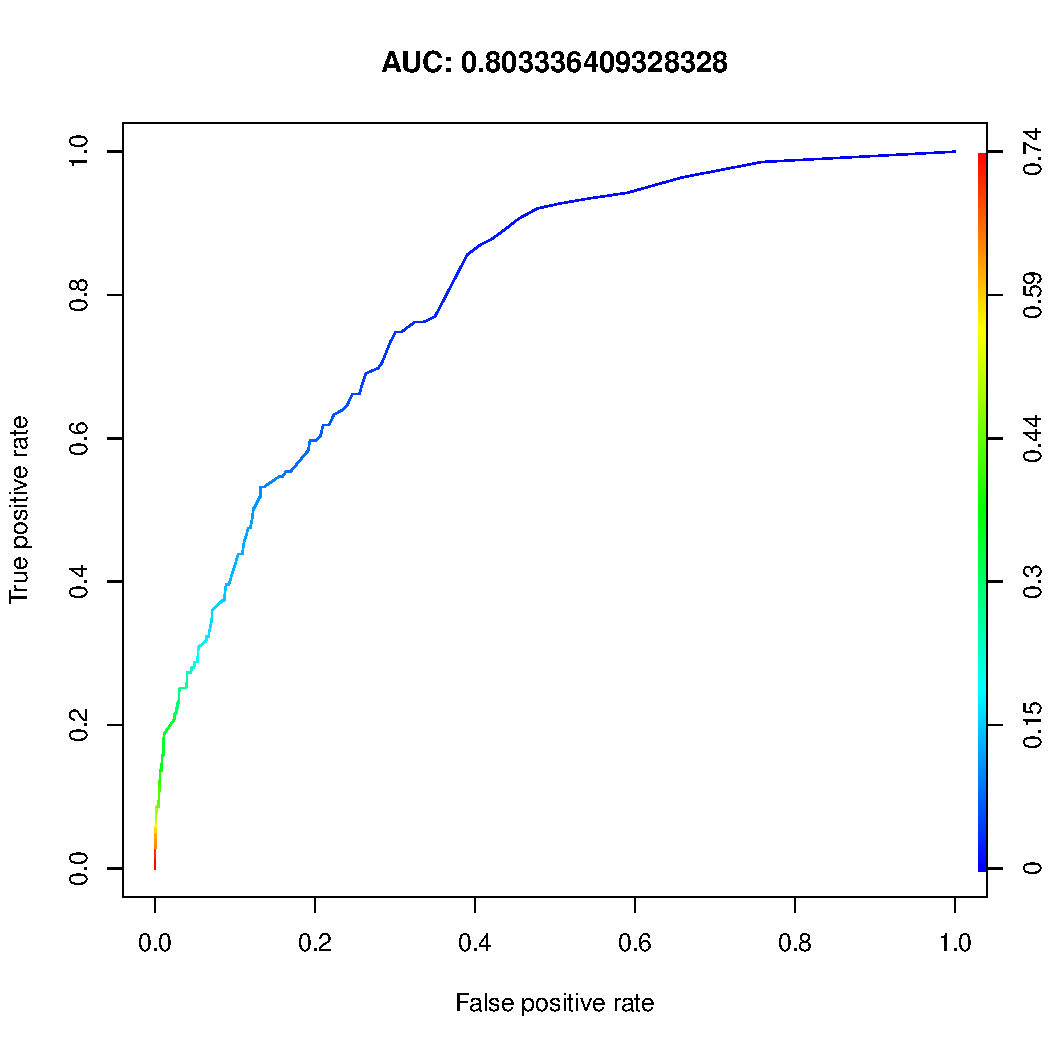
\includegraphics[width=.32\textwidth]{images/ml/random_forest/CrossValidationRF/valid/auc_2}
	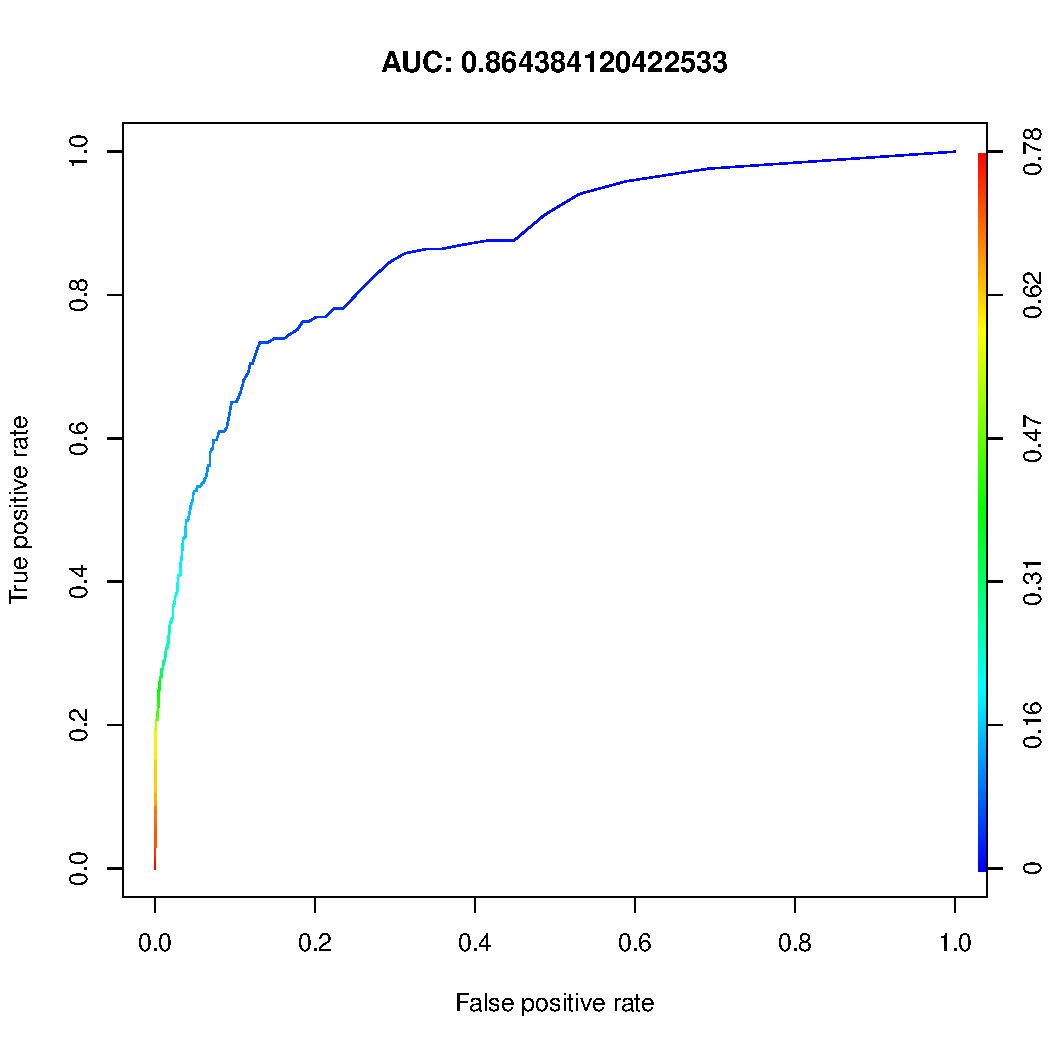
\includegraphics[width=.32\textwidth]{images/ml/random_forest/CrossValidationRF/valid/auc_3}
	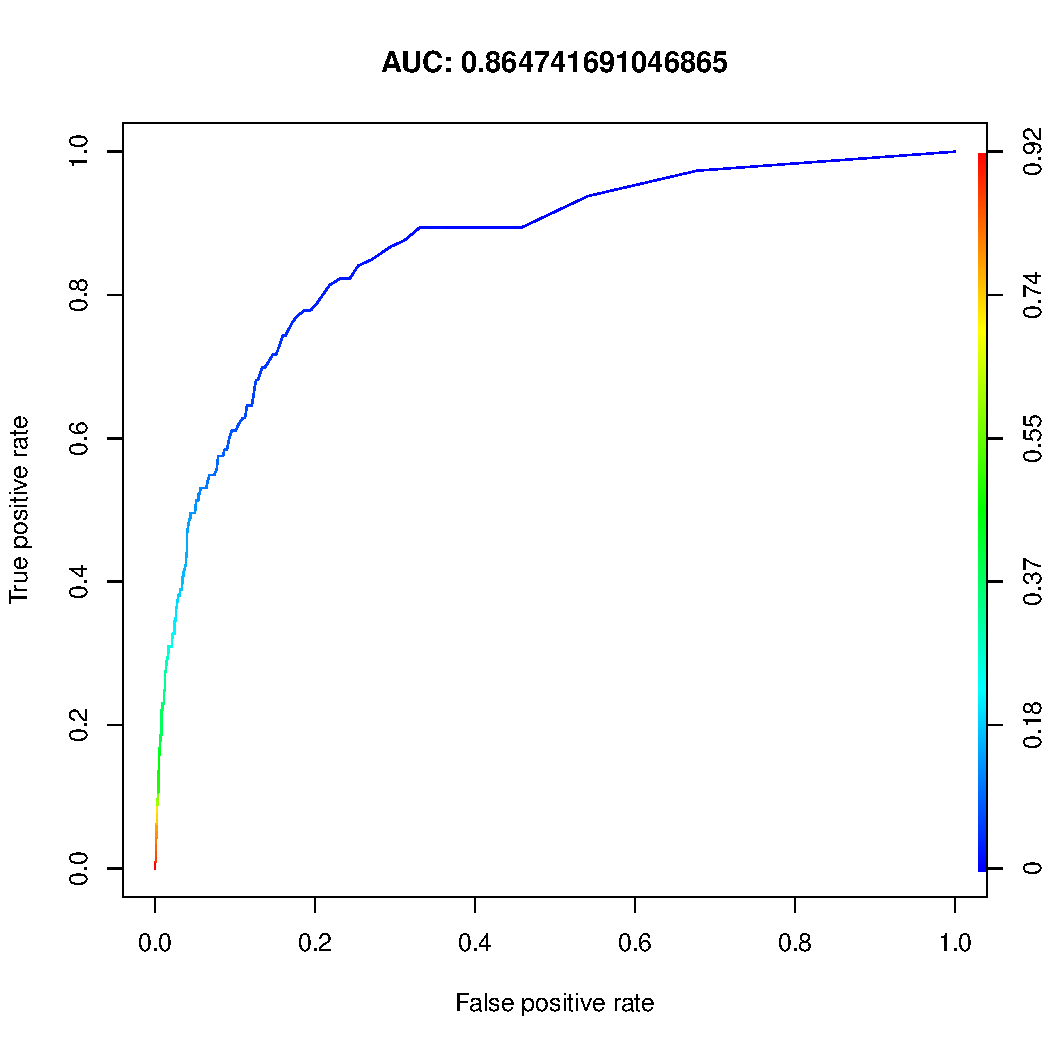
\includegraphics[width=.32\textwidth]{images/ml/random_forest/CrossValidationRF/valid/auc_4}
	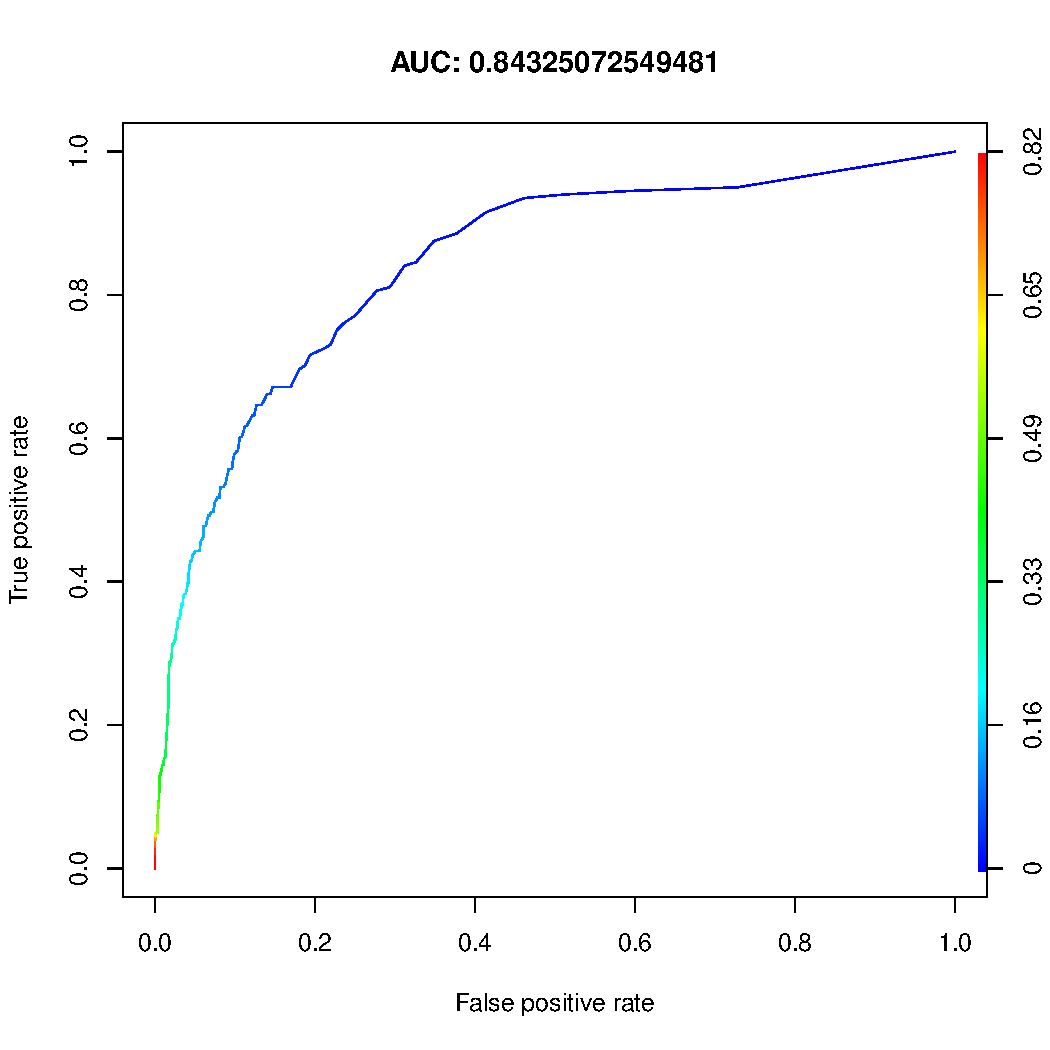
\includegraphics[width=.32\textwidth]{images/ml/random_forest/CrossValidationRF/valid/auc_5}
	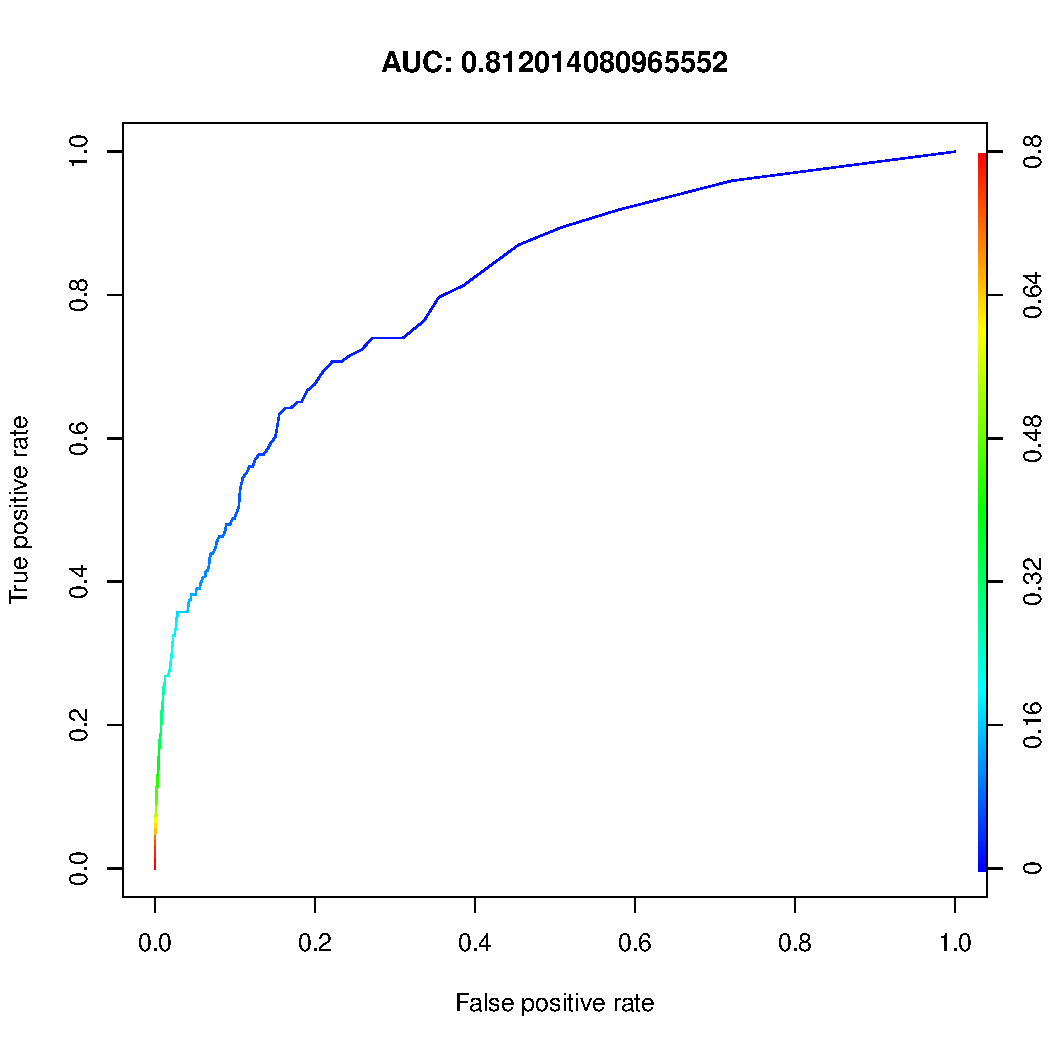
\includegraphics[width=.32\textwidth]{images/ml/random_forest/CrossValidationRF/valid/auc_6}
	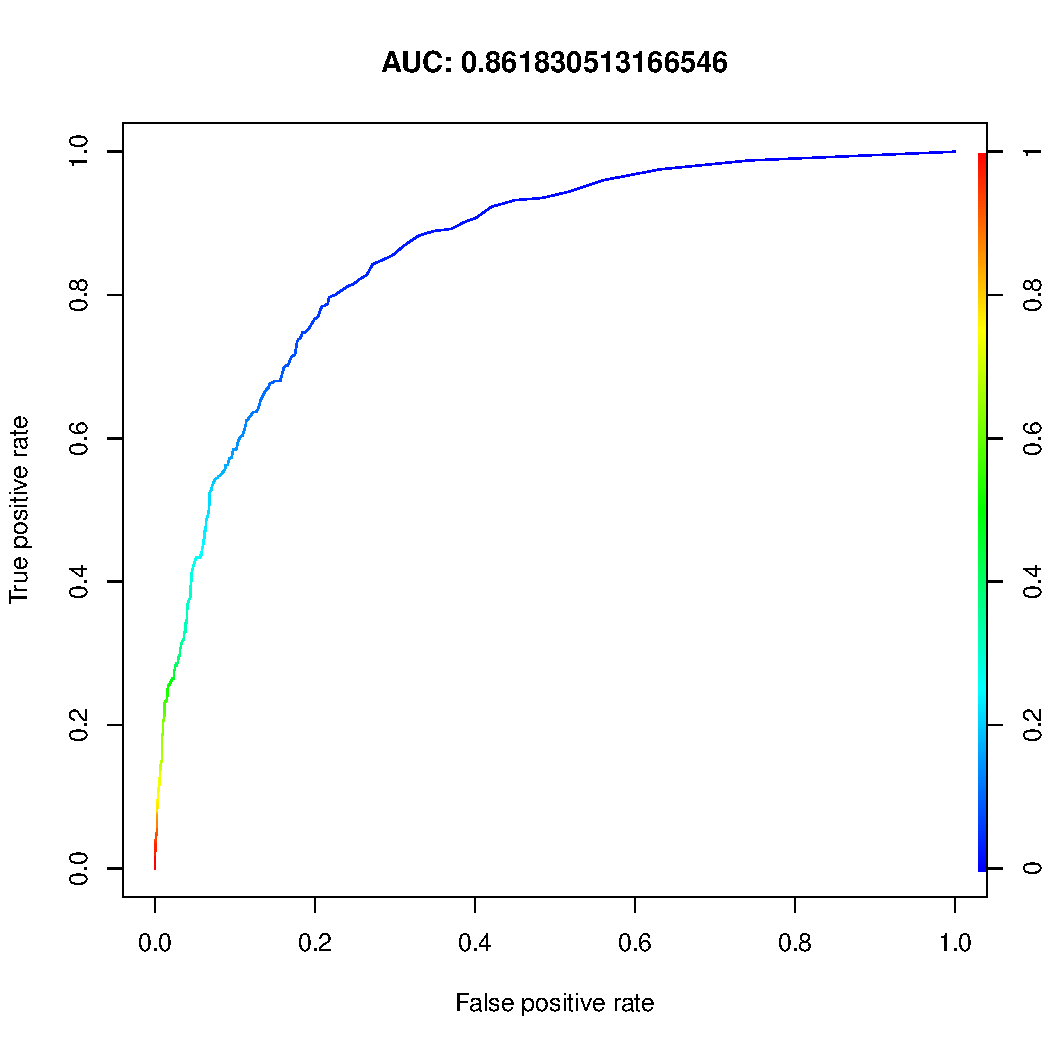
\includegraphics[width=.32\textwidth]{images/ml/random_forest/CrossValidationRF/valid/auc_7}
	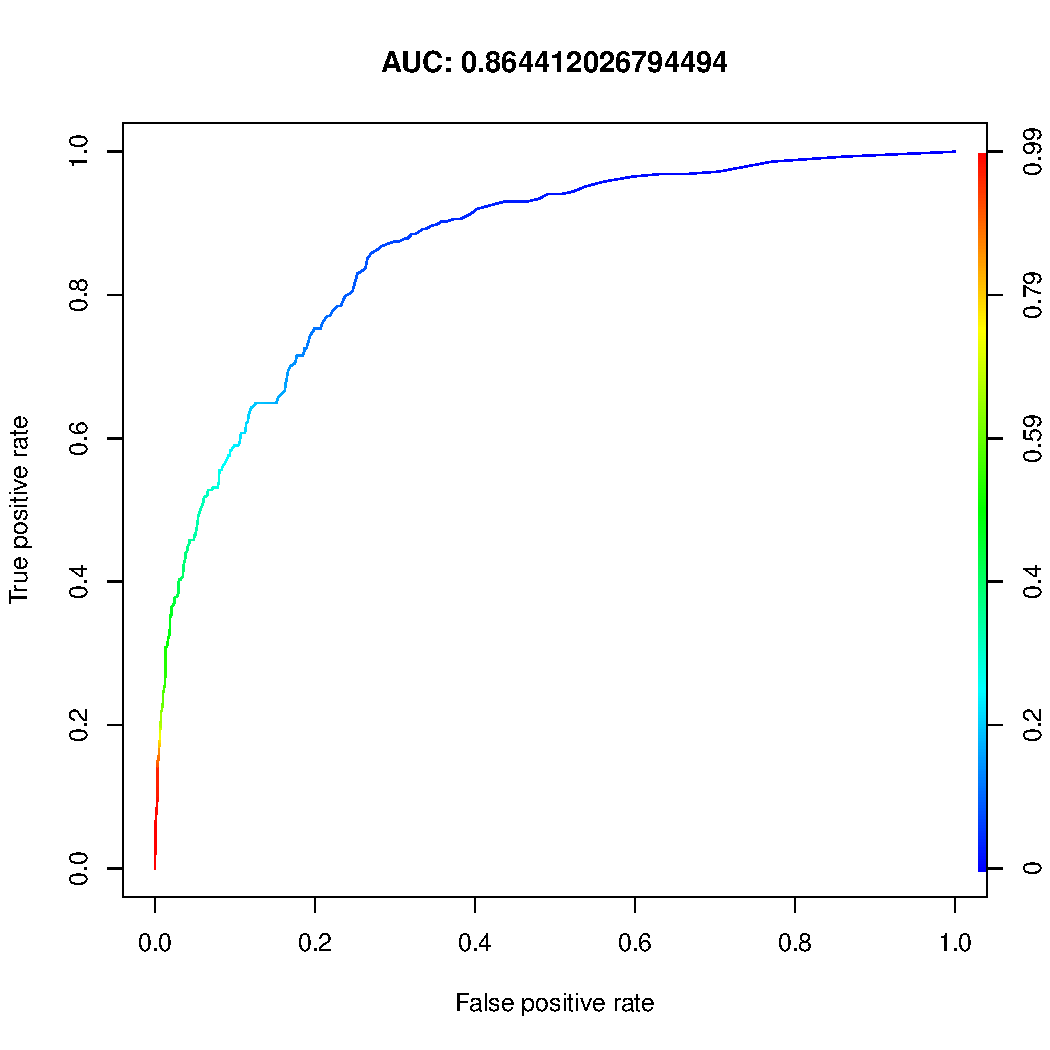
\includegraphics[width=.32\textwidth]{images/ml/random_forest/CrossValidationRF/valid/auc_8}
	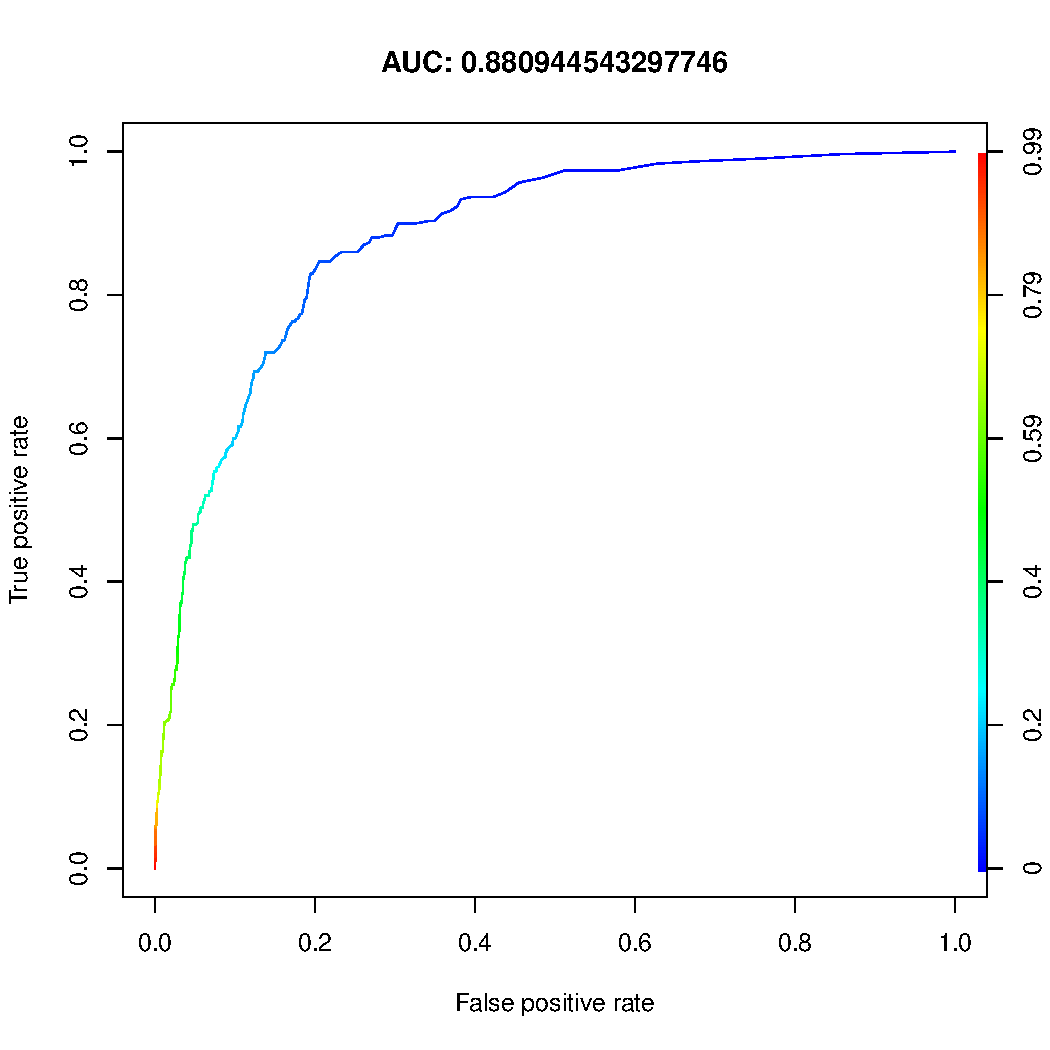
\includegraphics[width=.32\textwidth]{images/ml/random_forest/CrossValidationRF/valid/auc_9}
	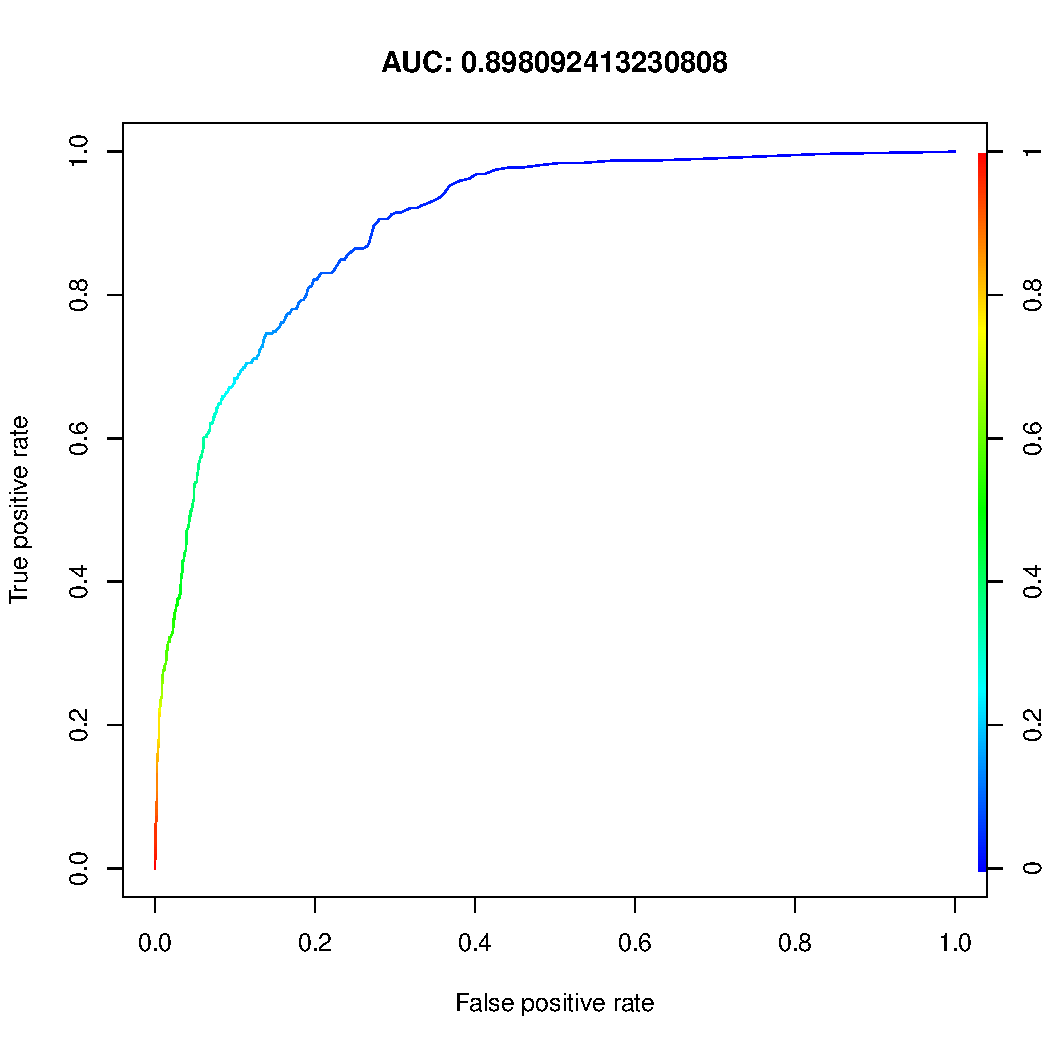
\includegraphics[width=.32\textwidth]{images/ml/random_forest/CrossValidationRF/valid/auc_10}
	\caption{ROC sul validation set}
	\label{fig:rf_cv_roc_valid}
\end{figure}

Possiamo vedere che in nessun fold il modello ha un valore di Area Under Curve 
(AUC) inferiore al valore 0,80, che viene considerato come un indice di buone 
prestazioni. Mediamente si ha un valore di 0,85.
